\documentclass[11pt,a4paper]{article}
\usepackage[francais]{babel}
\usepackage[utf8]{inputenc}
\usepackage[T1]{fontenc}

\usepackage{amsmath}
\usepackage{amsfonts}
\usepackage{amssymb}
\usepackage{makeidx}
\usepackage{graphicx}
\usepackage[left=1.cm,right=1cm,top=1cm,bottom=2cm]{geometry}
\usepackage{tabularx}
\usepackage{epstopdf}
\usepackage{booktabs}
\usepackage{threeparttable}
\newcommand{\Angstrom}{\textup{\AA}}
\usepackage{longtable}
\usepackage{multirow}
%\usepackage[labelfont=bf]{caption}
\usepackage{multicol}
\usepackage{pbox}
%\usepackage{hyperref}
%\usepackage{cleveref}
%\usepackage[pdftex]{graphicx}
\usepackage{epstopdf}
\usepackage{float}
\usepackage{rotating}
\usepackage{array}
 
%\usepackage{lmodern}
%\usepackage{mathpazo}
%\usepackage{microtype}
%\usepackage{geometry}
\usepackage{caption}
%\usepackage{xkeyval}
%\usepackage{subfigure}
\usepackage[dvipsnames]{xcolor}
\usepackage{sectsty}
%\usepackage{selinput}
\usepackage{babel}
%\usepackage{ulem}
%\usepackage{mathtools}
\usepackage{framed}
%\graphicspath{{/Users/bertrandsiboulet/Documents/minutes/figures/}}
\DeclareGraphicsExtensions{.eps,.pdf}
 
\newcolumntype{?}{!{\vrule width 2pt}}
%\usepackage[toc,page]{appendix}
\chapterfont{\color{NavyBlue}}
%\titleformat{\chapter}[display]
%{\normalsize \huge \color{NavyBlue}}%
%{\flushright \normalsize \color{Black}}%
%{\MakeUpperCase{\chaptertitlename}\hspace{1ex}%
%{\fontfamiliy{mdugm}\fontsize{60}{60}\selectfont\thechapter}}%
%{10pt}%
%{\bfseries\huge}%
\sectionfont{\color{BrickRed}}
\subsectionfont{\color{Maroon}}
\subsubsectionfont{\color{Red}}
\paragraphfont{\color{OrangeRed}}
%\renewcommand{\familydefault}{\sfdefault}
%\usepackage{geometry}
%\usepackage{pgfplots}
\makeatletter
\renewcommand\paragraph{\@startsection{paragraph}{4}{\z@}%
{-2.5ex\@plus -1ex \@minus -.25ex}%
{1.25ex \@plus .25ex}%
{\normalfont\color{OrangeRed}\normalsize\bfseries}}
\makeatother
 
\setcounter{secnumdepth}{4}
\setcounter{tocdepth}{4}
\bibliographystyle{elsarticle-num}
 
\usepackage[automark]{scrpage2}
\setheadsepline{.4pt}
\usepackage{listings}
\makeatletter
\renewcommand\tableofcontents{%
    \@starttoc{toc}%
}
\makeatother
\renewcommand{\arraystretch}{1.2}
%commands used in my current template
\newcommand*\mycommand[1]{\texttt{\emph{#1}}}
\newcommand*{\doi}[1]{\href{http://dx.doi.org/#1}{doi: #1}}
\newcommand{\comment}[1]{\textit{\textcolor{Red}{#1}}}
\newcommand{\addref}[1]{\textit{\textcolor{Red}{Add reference!}}}
\newcommand{\sub}[1]{\textsuperscript{#1}}
 
 
\begin{document}
\begin{flushleft}
\Large \textcolor{BrickRed}{\textsc{\textbf{Travaux d'Initiative Personnelle Encadrés}}} \\
\Huge \textcolor{BrickRed}{\textsc{\textbf{Informatique et prévisions météorologiques }}} \\[0.5cm]
\Large \textcolor{BrickRed}{\textsc{\textbf{Concours CPGE 2021 \\[0.5 cm]}}}
\hrule \textcolor{White}{-} \\[0.1cm]
%\Large \textcolor{BrickRed}{\textsc{\textbf{Concours CPGE 2021 \\}}}
\Large \textsc{Hélène Siboulet MP} \\
\Large \textsc{Juin 2021} \\[0.5cm]
\hrule
\end{flushleft}
\tableofcontents
\section{Présentation} 
%%%%%%%%%%
La prévision consiste à prévoir, c'est-à-dire à \og voir avant\fg{}. Il s'agit donc, à partir de ce que l'on sait à un moment donné, de savoir ce qui se passera à un moment ultérieur, avec la meilleure probabilité. En effet, à part les phénomènes déterministes, comme par exemple le mouvement des solides à court terme, on ne peut avoir que des indications probabilistes. C'est un problème universel, qui s'applique à l'économie, la politique, la vie privée, et aussi bien sûr aux prévisions météorologiques.\\   
%Définir l'intelligence en général est très compliqué. Voici une définition simple pour ce rapport~: observer-se souvenir-faire un modèle de prévision. Il existe un dicton météorologique~: "Quand la neige ne fond pas, c'est quelle en attend d'autre." Ce dicton est confirmé par les observations. Comme les masses d'air en France circulent d'ouest en est, la neige tombe d'abord sur un front d'air chaud -air froid, puis reste sous l'air froid, et tombe encore sur le front air froid - air chaud. On peut dire que ce dicton est une forme d'intelligence. Ce travail de TIPE est semblable, puisqu'il existe des paramètres (température et humidité), ils sont sur des bases, et ce travail développe une utilisation de ces données.  On peut parler d'intelligence artificielle. \\
La prévision repose sur deux éléments : des données disponibles à un moment, et des théories ou des modèles qui permettent d'utiliser ces données. \\
Les processus météorologiques sont tout à fait chaotiques. Cela signifie que des incertitudes minimes à un instant donné peuvent avoir des conséquences très fortes sur le déroulement. En fait, ces incertitudes n'empêchent pas de prévoir à court terme, par exemple pour le lendemain, mais elles rendent difficiles les prévisions au delà de deux semaines. \\
Si les processus météorologiques sont chaotiques à moyen terme, ils sont au contraire extrêmement stables dès lors que on les analyse en moyenne. Par exemple, Milankovitch a prévu que les variations de trois paramètres~-excentricité, obliquité et précession~-auraient des effets périodiques sur les glaciations. Milankovitch a fait apparaître des périodes de 20~000, 40~000 et 100~000 ans, ce qui a été confirmé expérimentalement par les mesures de $\delta O_{18}$ dans les carottes glaciaires de Vostock, en 1976. Ces résultats montrent que, en faisant des moyennes sur une centaine d'année, on a des tendances très claires d'évolution des températures, alors qu'il est difficile de prévoir la température dans deux semaines.   
 
Dans ce documents, nous allons faire un bref état de l'art des méthodes de prévision météorologiques utilisées, et proposer une méthode basée sur l'intelligence artificielle. Nous verrons que ces deux approches sont tout à fait différentes. Nous collectons une base de données, nous élaborons une méthode avec de nombreuses variantes. Chaque variante est évaluée numériquement, c'est à dire par comparaison des prévisions avec un ensemble de données qui ont été placées en dehors des données d'entrées.

 \vspace {0.6cm}
Les prévisions météorologiques ont beaucoup d'enjeux, elles permettent notamment :
\begin {enumerate}
\item aux pilotes d'avion et aux marins de savoir si leur trajet est réalisable, de connaitre la quantité de carburant à prendre et de choisir l'itinéraire le plus adapté
\item aux agriculteurs de savoir quand arroser, quelle quantité d'eau est nécessaire, quand labourer, planter ou récolter 
\item d'organisation d'activités ou d'évènements en plein air
\item de gérer des risques liés au climat par exemple lorsqu'il y a du verglas, de la neige, une canicule ou une tempête
\end{enumerate}

 
\section{État de l'art}
%Méthode la plus courante de prévision météo selon Jean Pailleux de Météo-France
%Modélisation de l'atmosphère par :
%\begin{enumerate}
%\item Équation du mouvement(Newton)
%\item $\frac{d\bold{V}}{dt} = \bold(g) - \frac{\bold{grad}p}{d} $
%\item Équation de continuité
%\item Thermodynamique
%\item Équation des gaz parfaits
%\item Équations de bilans de constituants: vapeur d’eau, eau liquide, ozone, etc...
%\end{enumerate}

Il existe plusieurs sortes de prévisions météorologiques : la prévision du temps qui fait des prédictions sur des périodes de quelques jours, la prévision saisonnière qui fait des prédiction sur l'échelle d'un moi ou de quelques mois et la prévision climatiques prédit l'évolution du climat sur plusieurs années.

Selon http://meteocentre.com/intermet/prevision/prevision\_emp.htm
les principales méthodes de prévision météorologiques sont :
\begin{enumerate}
\item La méthode de la persistance qui prédit que demain il fera le même temps qu'aujourd'hui. Elle fonctionne bien dans certaines régions où les conditions météorologiques varient lentement comme	l'Egypte ou les déserts des États-Unis. Elle fait de bonnes prévisions sur des périodes de un ou deux jours ainsi et est efficace pour prédire des tendance sur des durées d'un moi (prévisions saisonnière). 
\item La méthode de la tendance qui étudie les déplacement de systèmes météorologiques tels que les dépressions, les anticyclones, les fronts et les zones de précipitation et suppose leurs emplacement futurs.
\item La méthode de l'analogie qui consiste à chercher des cas dans le passé qui ressemblent aux conditions météorologiques actuelles et à supposer que ces conditions évolueront de la même manière.
\item La méthode numérique est la plus utilisée actuellement. On mesure les différentes paramètres ce qui nous donne l'état initial. Les lois physiques prédisent ensuite l'évolution du système. Il s'agit d'une simulation physique de l'atmosphère. L'article de Pailleux \cite{PAILLEUX}
 propose notamment une simulation basée sur les équations hydrodynamique suivantes : \begin {enumerate}
\item Principe fondamental de la dynamique
\item Équation de continuité
\item Premier principe de la thermodynamique
\item Loi des gazs parfaits
\item Équation bilan des constituants
\end {enumerate}
Cette méthode requiert :
\begin{enumerate} 
\item La découpe de l'atmosphère dans une grille en trois dimensions. Plus la grille est large plus les calculs sont rapides et moins ils sont précis.
\item L'intégration des équations précédentes. Le plus souvent en approximant la dérivée des différents paramètres comme constant sur un petit intervalle de temps dt. Pour que le modèle fonctionne il faut que dt soit suffisamment petit pour que les paramètres changent peu sur dt et en particulier que les systèmes météorologiques se déplacent de moins d'une case dans la grille.
\item Une puissance numérique très élevée. Par exemple, le calculateur de Météo-France ATOS Sequana XH2000 possède une puissance de 100 pétaFLOPS. 
\end {enumerate}
\end{enumerate}

On trouve sur internet d'autre types d'outils de prévision tels que des réseaux de neurones, des algorithmes génétiques, de la logique floue et des réseaux bayésiens %et d'autres modèles probabilistes
 (voir Das2017).

Toutes ses méthodes peuvent être exploités différemment : pour faire des prévisions déterministes ou probabilistes. Étant donné la précision des méthodes actuelles, la méthode déterministe peut être utilisée pour des échéances de trois à quatre jours. Faire des prévision probabilistes, aussi appelées prévisions d'ensemble, consiste à donner plusieurs prévisions à partir d'états initiaux proches. Ces états initiaux sont choisis de sorte à refléter l'incertitude des prévision. Il faut ensuite comparer les différentes prévisions pour déterminer quels sont les scénarios les plus probables et en cas de risques liés au climat quels sont les pires scénarios (voir Meteofrance).

\vspace{0.6cm}
Nous avons choisi pour ce TIPE de privilégier différentes approches de modélisation mathématique.

\section{Recherche de données}

Nous avons trouvé une base de donnée sur  : \\
https://donneespubliques.meteofrance.fr/?fond=produit\&id\_produit=90\&id\_rubrique=32. \\
Elle contient les relevés de 62 stations en France Métropolitaine et en France d’Outre mer
de 1996 à 2020  (avec certaines mesures manquantes : pas plus de 80 en une année soit l'équivalent de dix jours sauf pour 2020)
avec un relevé toutes les trois heures soit huit relevés par jour.
Les donnees sont : la température, l'humidité, la direction et la force du vent, la pression atmosphérique, la hauteur de précipitations, le temps sensible, la description des nuages, la visibilité.
Chaque fichier couvre un mois et toutes les stations. \\
Nous avons collecté sur le site avec Webbot. \\
Nous avons décompression les fichiers vers le format csv décompressé. \\
Nous avons trié les données par station. \\

\section{Modèles de prévision sur une station : analyse de la température et de l'humidité}

Extraction des données de température et d'humidité de Clermont-Ferrand au au format json \\
Les annees 2008, 2019 et 2020 sont retirées de la base d'entrainement et serviront de base de test\\
\begin{figure} [!h]
\centering
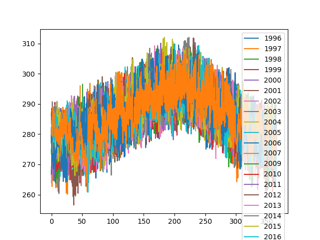
\includegraphics[width=0.48 \textwidth]{./imagesTIPE/temperature.png}\quad
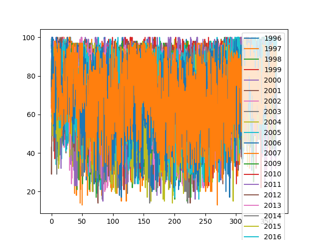
\includegraphics[width=0.48 \textwidth]{./imagesTIPE/humidite.png}
\caption{\label{fig:190101Lolita} Courbes de température et d'humdité de la base d'apprentissage : Clermont-Ferrand}
\end{figure}

Comment estimer la valeur d'un ensemble de prévisions~? On calcule l'écart type entre nos prévisions et les températures mesurées. Cela permet d'estimer la valeur des prévisions, mais à condition d'avoir une valeur de comparaison. Nous utilisons pour cette valeur l'écart type des températures.
 \\ Calcul de valeurs utiles de la base de donnée : quartiles, medianne, moyenne, écart type.\\ 
%Température :  $Q1 = 6.39{}^{\circ}C  \quad Q3 = 17.4{}^{\circ}C$   soit un intervalle de $11{}^{\circ}C $ \\
%Humidité :  $ Q1 = 59.0\%  \quad  Q3 = 85.0\% $ soit un intervalle de $26\% $ \\
\begin{tabular}{llllll}\hline\hline
Température& $Q1 = 6.39{}^{\circ}C$ &$ me = 11.9 {}^{\circ}C$ & $Q3 = 17.4{}^{\circ}C $&$ m= 12.0 $ & $\sigma = 7.91 {}^{\circ}C$ \\
Humidité    &   $ Q1 = 59.0\%$           &$  me = 73.0\%  $           & $Q3 = 85.0\%.           $& $ m=71.2  $ & $\sigma = 17.1 \% $ \\
\hline 
\end{tabular} 



%moyenne

\subsection{Premier modèle : Moyenne de la température et de l'humidité par jour de l'année et par heure }
Nous considérons dans ce modèle que la température et l'humidité sont cycliques de période un an et nous prévoyons qu'un jour donné à une heure donnée il fera la moyenne des température et humidité qu'il a fait ce jour ci lors des années précédentes.
Calcul des moyennes sur la base d'entrainement : \\

\begin{figure} [!h]
\centering
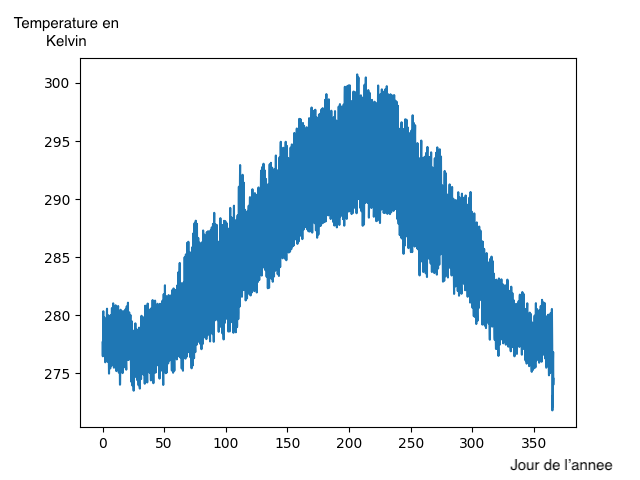
\includegraphics[width=0.48 \textwidth]{./imagesTIPE/moyenneT.png}\quad
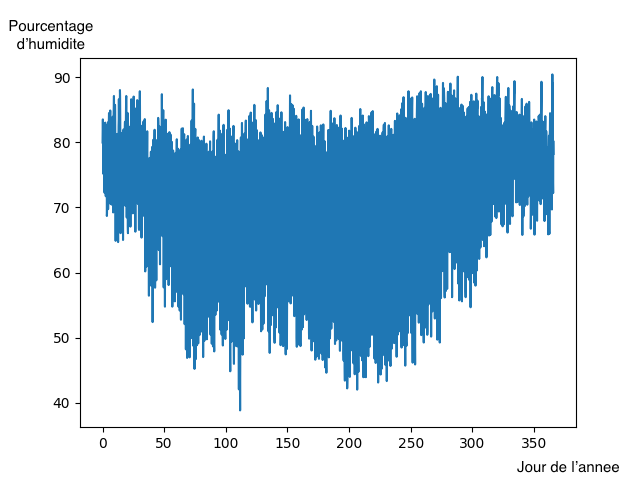
\includegraphics[width=0.48 \textwidth]{./imagesTIPE/moyenneH.png}
\caption{\label{fig:190101Lolita} Courbes des moyennes de température et d'humidité de la base d'apprentissage par jour et heure}
\end{figure}

\begin{tabular}{lll}\hline
\hline
Écart type de la température& $4.28{}^{\circ}C$\\
Écart type de l'humidité       &  $ 14.8\% $\\
\hline 
\end{tabular}

%persistance

\subsection{Deuxième modèle : Modèle de la persistance journalière}
 La température et l'humidité varient selon des cycles jours nuit. Nous considéreront ici que ces paramètres varient peu d'un jour sur l'autre. Nous prédisions donc que dans x jours il fera la même température que x jours avant à la même heure.
\begin{tabular}{lllllll}\hline
\hline
Prévision à x jour                  &1                         &2                         &3                           &4                         &5                          &6 \\
Écart type de la température& $2.59{}^{\circ}C$& $11.1{}^{\circ}C$& $12.3{}^{\circ}C$& $12.9{}^{\circ}C$& $13.1{}^{\circ}C$& $13.0{}^{\circ}C$\\
Écart type de l'humidité       &  $ 15.0\% $         &  $ 16.8\% $         &  $ 17.5\% $        &  $ 17.7\% $         &  $ 17.6\% $         &  $ 17.7\% $\\
\hline 
\end{tabular}

%cosinus

\subsection{Troisième modèle : Approximation de la courbe des températures par une somme de fonctions sinusoïdales}
À priori les conditions météorologiques sont cycliques par rapport à l'année et au jour. Nous pouvons donc nous demander si il est judicieux de modéliser ses paramètre par une somme de sinusoïdes. Nous réalisons donc une
transformation de Fourier pour nous demander si la méthode est appropriée. \\
Pour réaliser une transformation de Fourier discrète, nous utilisons la bibliothèque numpy sur python qui utilise la formule suivante :  \\
$ A_{k}  = \displaystyle { \sum_{m=0}^{n-1}} a_{m} exp(-2\pi i \frac{mk}{n} ) $ avec $k = 0, ... , n-1 $   \\ 
\vspace {0.3cm}
\begin{figure} [!h]
\centering
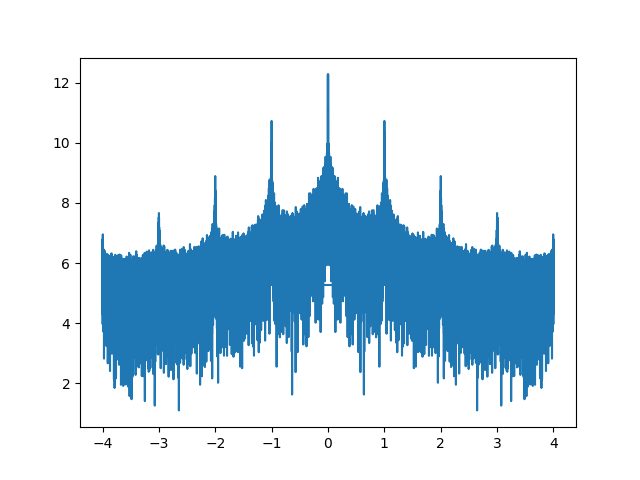
\includegraphics[width=0.48 \textwidth]{./imagesTIPE/fftT.png}\quad
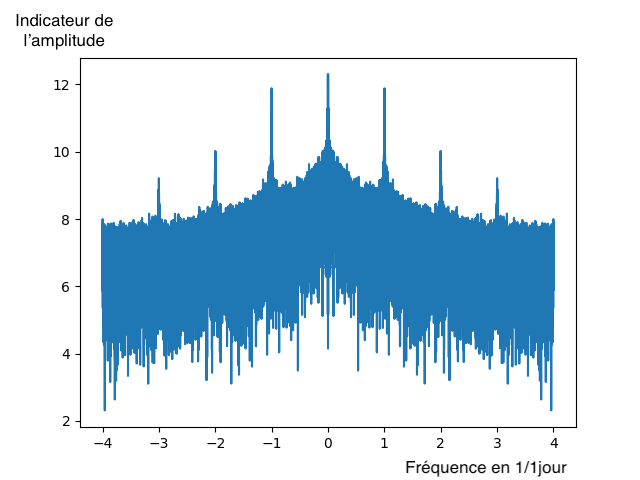
\includegraphics[width=0.48 \textwidth]{./imagesTIPE/fftH.png}
\caption{\label{fig:190101Lolita} transformation de Fourier discrète de la température et de l'humidité de la base d'entrainement}
\end{figure}
\begin{figure} [!h]
\centering
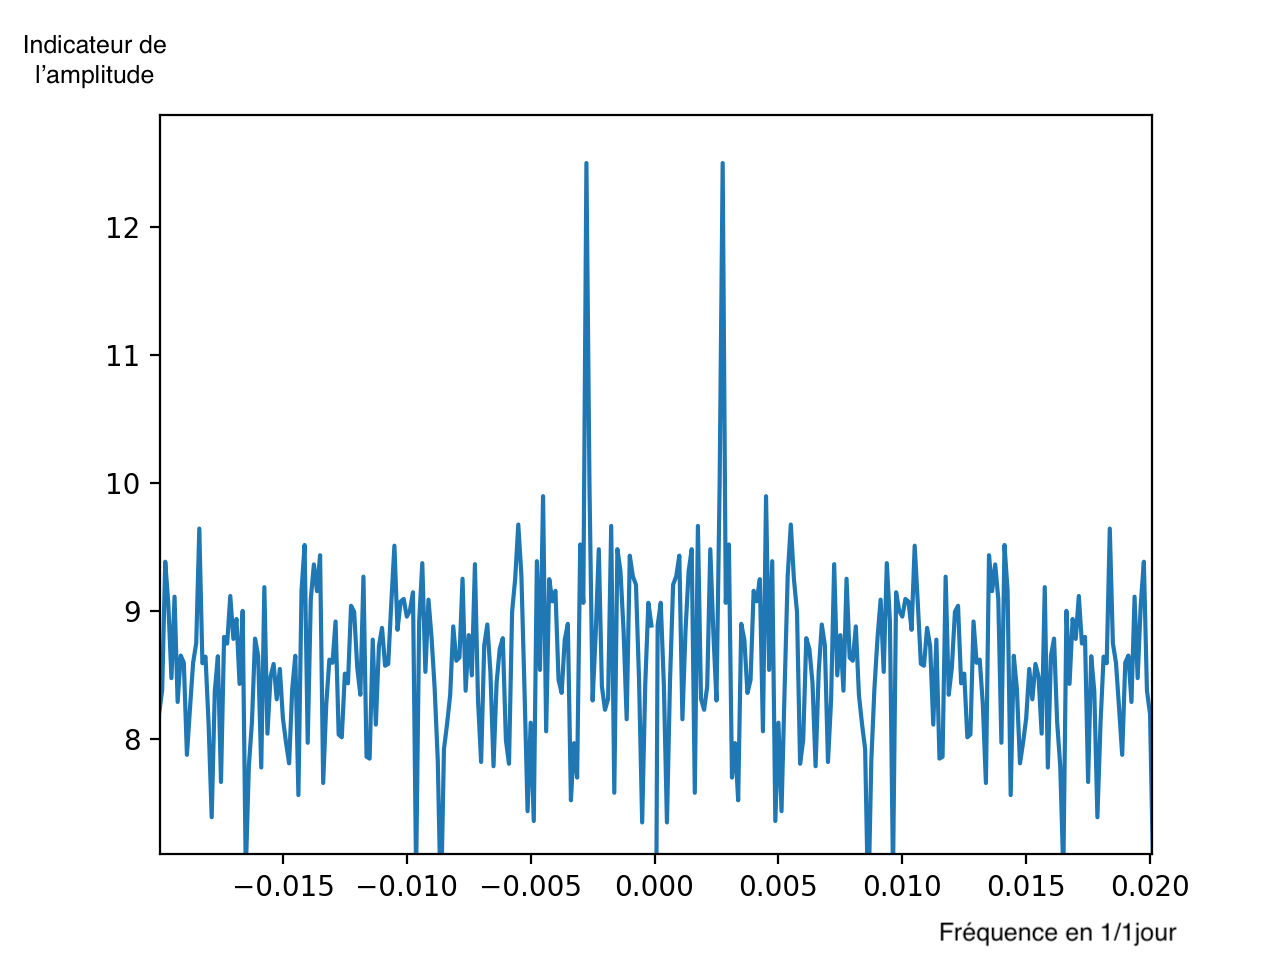
\includegraphics[width=0.48 \textwidth]{./imagesTIPE/fftTZ.png}\quad
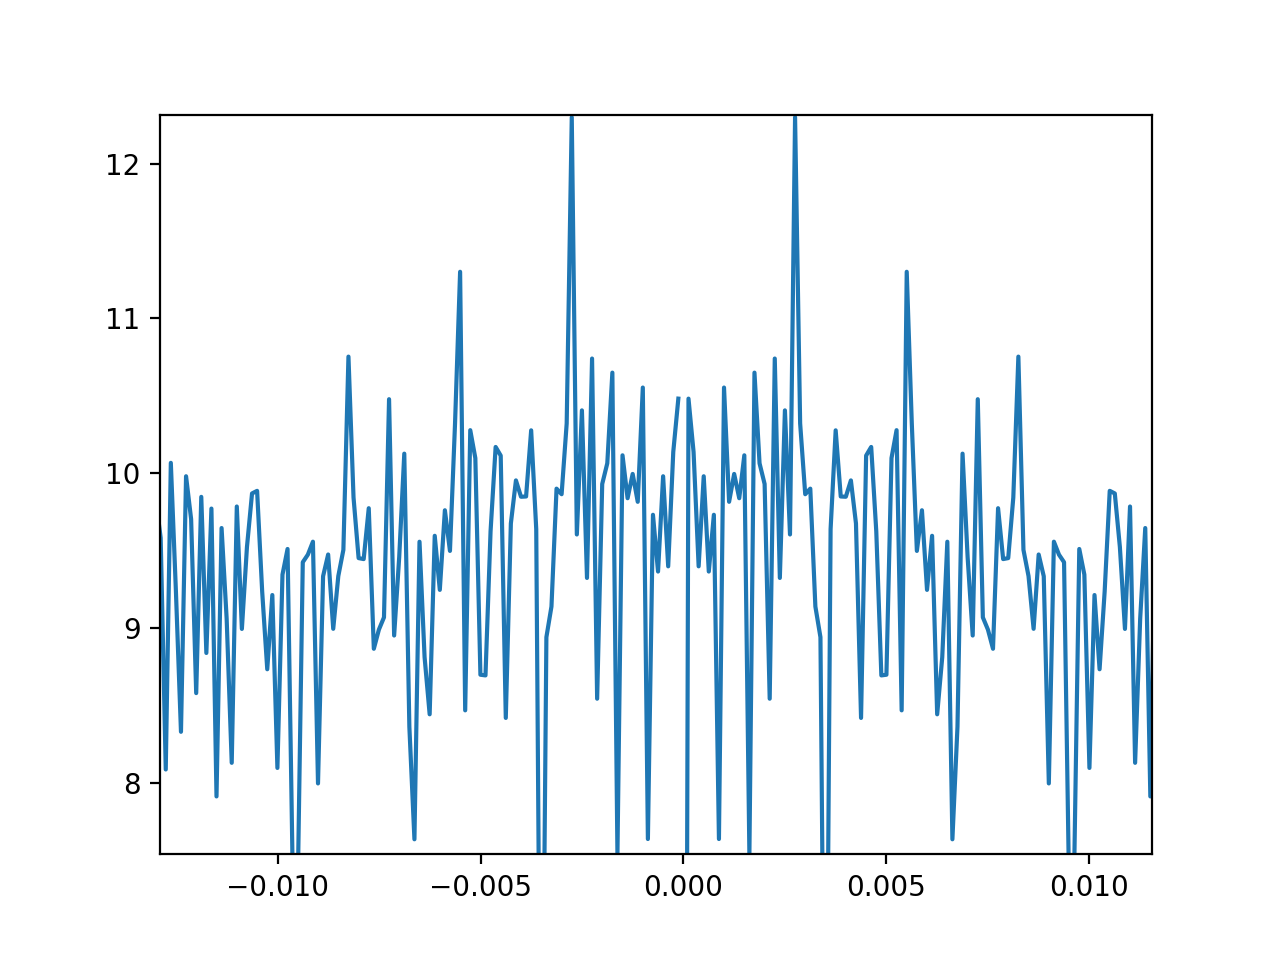
\includegraphics[width=0.48 \textwidth]{./imagesTIPE/fftHZ.png}
\caption{\label{fig:190101Lolita} transformation de Fourier discrète de la température et de l'humidité de la base d'entrainement zoomées sur 0 }
\end{figure}

Nous concluons que la méthode est appropriée. \\
Sur les deux courbes on observe des pics aux fréquence de 1/(365 jours) et 1/(1jour) ainsi que des harmoniques de ses fréquences.
On approxime donc les paramètres par des fonctions de la forme : \\
 $f(t) = A cos (\omega_{1} t + \phi_{1}) + B cos (\omega_{2} t + \phi_{2}) + C$  \\
$g(t) = A cos (\omega_{1} t + \phi_{1}) + B cos (\omega_{2} t + \phi_{2}) + C + D cos (\omega_{3} t + \phi_{3}) + E cos (\omega_{4} t + \phi_{4})$ \\
$h(t) = A cos (\omega_{1} t + \phi_{1}) + B cos (\omega_{2} t + \phi_{2}) + C + D cos (\omega_{3} t + \phi_{3}) + E cos (\omega_{4} t + \phi_{4}) + F cos (\omega_{5} t + \phi_{5}) + G cos (\omega_{6} t + \phi_{6})$ \\ 
Avec $\omega_{1} = 2 \pi$ (période journalière) , $\omega_{2} = 2 \pi /365$ (période annuelle), $\omega_{3} = 4 \pi$ (période demi-journalière), $\omega_{4} = 4\pi/365 $  (période semi annuelle), $\omega_{5} = 6 \pi$ (période du tiers de journéé), $\omega_{6} = 6\pi/365 $  (période du tiers d'année)\\

Il faut ensuite déterminer les valeurs de des coefficients et des déphasage. On utilise alors la méthode du gradient :
\begin{itemize}
\item On crée une fonction écart qui calcule l'écart type entre les prévisions et les valeurs de la base d'entrainement en fonction des coefficients et des déphasages. On cherche alors à déterminer le minimum de écart.
\item On initialise les paramètres (déphasages et coefficient) à une valeur approximative
\item On dérive écart par rapport à chaque paramètre
\item On modifie chaque paramètre X en faisant X = X - dX
\item On répète les deux points précédents un grand nombre de fois
\end{itemize}

Nous testons la fonction obtenue sur la base de test en calculant l'écart type.

\begin{tabular}{llll}\hline
\hline
Fonction                             &f                         &g                       &h \\
Écart type de température & $4.38{}^{\circ}C$   & $1{}^{\circ}C$   &  $1{}^{\circ}C$ \\ 
Écart type de d'humidité    & $15.3\%$   & $1\%$   &  $1\%$   \\   
\hline 
\end{tabular}





























\section{Exemples Latex}
\subsection{subsection}
\subsubsection{q;,c}
%Donner un référence : \cite{Adler:1964aa}
\subsubsection{Donner des figures}

%%%%%%
\begin{figure}
  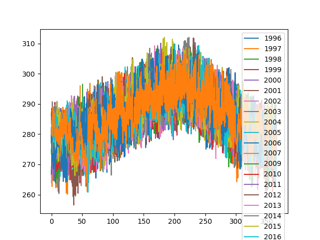
\includegraphics[width=0.48 \textwidth]{./imagesTIPE/temperature.png}\quad
\end{figure}
\begin{figure}
  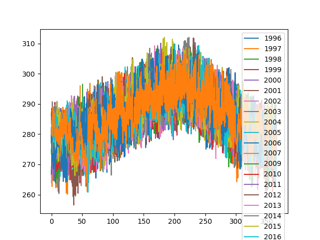
\includegraphics[width=0.48 \textwidth]{./imagesTIPE/temperature.png}\quad
\end{figure}
%%%%%
%%%\begin{figure}
%\centering
%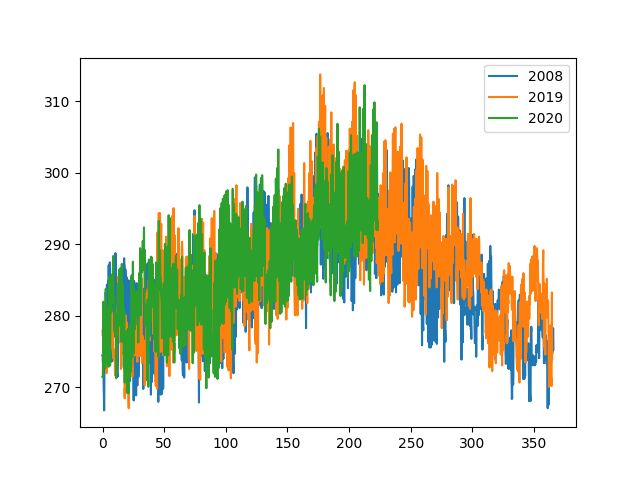
\includegraphics[width=0.48 \textwidth]{/Users/siboulet/Desktop/imagesTIPE/temperature.png}\quad
%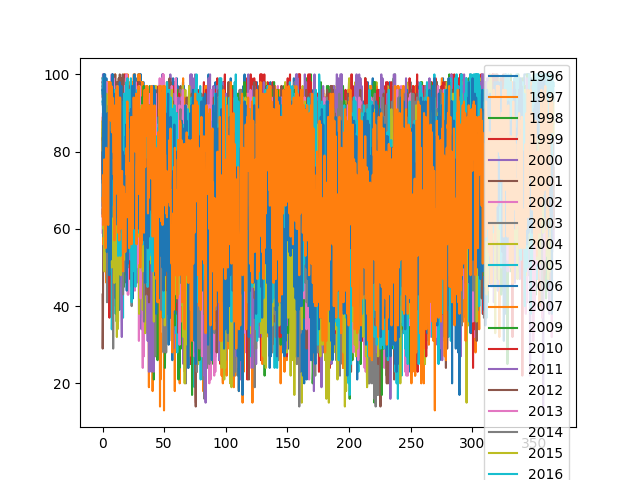
\includegraphics[width=0.48 \textwidth]{/Users/siboulet/Desktop/imagesTIPE/humidite.png}
%\caption{\label{fig:190101Lolita} A droite : pointe AFM / surface d'eau, à gauche :  Coalescence de gouttes d'eau }
%\end{figure}

\subsubsection{Citer des figures}
Je cite la figure \ref{fig:190101Lolita}
%%%%%
\subsection{Placer un tableau}
\begin{table}[ht]
\begin{tabular}{cccc}\hline
\hline
Ow& 15.99945& -0.8476&SPCE\\
Hw&  1.0079 &  0.4238&SPCE\\
Na& 22.9897 &  1.0000&\\         
Cl& 35.45   & -1.0000&\\
Os& 15.9994 & -1.000 &\\   
Ti& 47.8670 &  2.000 &\\  
\hline 
\end{tabular}                     
\caption{\label{MonTableau}, Charges for Ti02/W/Na/Cl}
\end{table}
\subsection{Citer un tableau}
Je cite mon tableau \ref{MonTableau}.


\section{Références}
\bibliography{./ref.bib}
%\begin{enumerate}
%\item Baselov, I., Vasileva, D., 2016. Numerical modeling of drop coalescence in the presence of soluble surfactants. J. Computational and Applied Mathematics 293, 7-19.
%\item Duchemin, L., Eggers, J., Josserand, C., 2003. Inviscid coalescence of drop. J. Fluid Mech. 487, 167-178.
%\end{enumerate}

\end{document}